\documentclass[a4paper,11pt]{article}

\usepackage[utf8]{inputenc} \usepackage[T1]{fontenc}
\usepackage{fancyhdr} \usepackage{graphicx,subfig} \usepackage{lastpage}
\usepackage{amssymb,amsmath} \usepackage{siunitx} \usepackage[nodayofweek]{datetime}
\usepackage[top=3.5cm,bottom=2.5cm,left=3cm,right=3cm,headheight=40pt]{geometry}
\usepackage{parskip} \usepackage{float} \usepackage{enumitem} \pagestyle{fancy}
\usepackage[colorlinks=true,allcolors=blue]{hyperref} \hypersetup{
	pdfauthor={Michaël Defferrard},
	pdftitle={Project stage 3: Interaction \& Animation},
	pdfsubject={Introduction to Computer Graphics}
}

\lhead{Introduction to Computer Graphics\\Project stage 3: Interaction \& Animation\\Group 19}
\chead{\hspace{2.5cm}EPFL\\\hspace{2.5cm}\shortdate\today\\\hspace{2.5cm}\thepage/\pageref{LastPage}}
\rhead{Michaël \textsc{Defferrard}\\Pierre \textsc{Fechting}\\Vu Hiep \textsc{Doan}}
\cfoot{}

\begin{document}


\section{Overview}

This report presents our advancement on the third part of the project : interaction and animation. During all the run of the project, we focused on code design and quality rather than quantity. It would have been impossible to implement every single idea we had about the project anyway.
%At this stage, we realized that we are better technicians than artists.


\section{Implementation}

\subsection{Basics}

\subsection{Advanced}


\section{Improvements on last stage}

\subsection{Code cleanup}

As this hand-in is the last opportunity to modify our code, we put great effort in cleaning it up, including comments. A great job was done to functionalize shader code. As a side effect, we did also discover some little mistakes.

\subsection{Lightning}

Phong shading was improperly implemented at stage 2. The material texture was only used for the ambient color. The diffuse and specular colors were fixed for all the terrain. Probably a reminiscent of stage 1. This is now fixed.

The light direction was defined to be the same for all the vertices, which is a directional light. This was changed to a spot light (or point light in the lightning context), to be coherent with shadowing.

We now retrieve material color properties from textures. The retrieved color is split across the three lightnings : ambient, diffuse and specular. For example, specular lightning coefficient is non-zero for water only.

\subsection{Vertices object}

To achieve better modulation, we have separated the vertices creation code into a class hierarchy. The \texttt{Vertices} base class is an abstract class, defining only virtual methods, which defines the interface. The \texttt{VerticesGrid} and \texttt{VerticesSkybox} inherit from it and implement the \texttt{generate} \texttt{draw} and \texttt{clean} methods which are specific to them. This design allows more than one \text{RenderingContext} object to share a \texttt{Vertices} object. The \texttt{Terrain} and \texttt{Shadowmap} makes use of this.

\subsection{Heightmap}

The heightmap texture was configured with the default heuristic for out-of-range values. This default is to wrap around the texture (\texttt{GL\_REPEAT}) which creates artifacts at the borders of the terrain (fig.~\ref{heightmap_artifacts}). Clamping the texture coordinates (\texttt{GL\_CLAMP\_TO\_EDGE}) to the [0,1] range eliminates the artifacts (fig.~\ref{heightmap_ok}).

\begin{figure}[ht]
	\centering
	\subfloat[With artifacts at the border]{
		\label{heightmap_artifacts}
		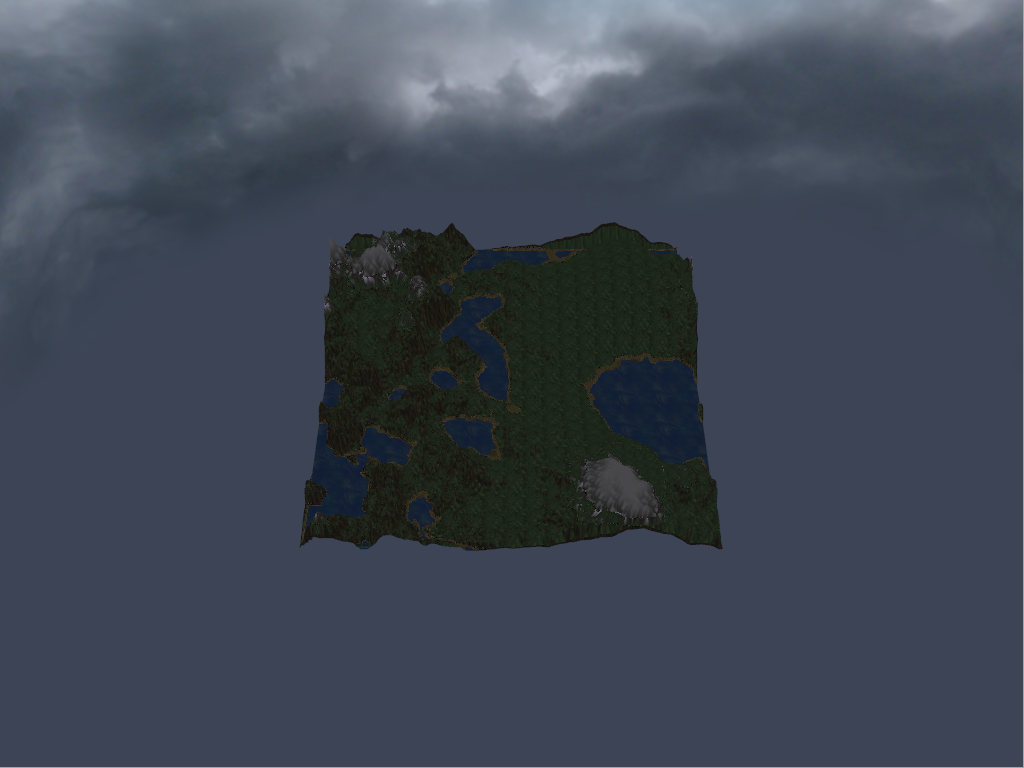
\includegraphics[height=4cm]{{{img_stage3/heightmap_artifacts}}}
	} \quad
	\subfloat[Without artifacts]{
		\label{heightmap_ok}
		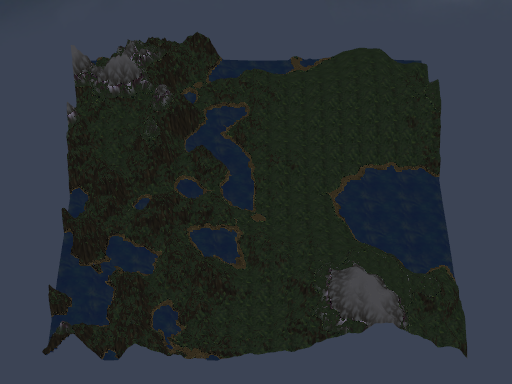
\includegraphics[height=4cm]{{{img_stage3/heightmap_ok}}}
	}
	\caption{Heightmap}
	\label{heightmap}
\end{figure}

\section{Results}


\end{document}
